\documentclass[12pt]{amsart}

\usepackage[margin=1in]{geometry}

\usepackage{amsmath,amssymb,amsthm}
\usepackage{hyperref}
\usepackage{tikz,tikz-cd}
\usetikzlibrary{calc}

\newtheorem{theorem}{Theorem}
\newtheorem{lemma}[theorem]{Lemma}
\newtheorem{proposition}[theorem]{Proposition}
\newtheorem{corollary}[theorem]{Corollary}
\newtheorem{conjecture}[theorem]{Conjecture}
\theoremstyle{definition} \newtheorem*{notation}{Notation}
\theoremstyle{remark} \newtheorem*{remark}{Remark}
\theoremstyle{remark} \newtheorem*{example}{Example}
\theoremstyle{definition} \newtheorem*{definition}{Definition}

\numberwithin{equation}{section}
\numberwithin{theorem}{section}

\renewcommand{\pmod}[1]{\left(\mathrm{mod}\,#1\right)}

\title{Arithmetic statistics course notes}
%~ \subtitle{Lecture I: Hilbert Irreducibility}

\author{Robert J. Lemke Oliver}
\date{\today}

\begin{document}

	\maketitle
	
	\setcounter{section}{1}
	
\section{Rings of integers and discriminants}
	
	We now turn to considering what will prove to be some of the most fundamental objects to this course, namely \emph{rings of integers}.  We begin with several definitions and lemmas.
	
	\subsection{Algebraic integers}
	
	\begin{definition}
		A number $\alpha \in \mathbb{C}$ is called an \emph{algebraic integer} if it is the root of a monic polynomial $f \in \mathbb{Z}[x]$.
	\end{definition}
	
	We've given this definition relative to roots of any monic integer polynomial because that's the definition that's easiest to check, but in fact, we could have defined it relative to irreducible polynomials only (as are usually considered when dealing with field extensions).
	
	\begin{lemma}
		A number $\alpha$ is an algebraic integer if and only if it is the root of an irreducible monic polynomial $f \in \mathbb{Z}[x]$.
	\end{lemma}
	\begin{proof}
		One direction is immediate: if $\alpha$ is the root of an irreducible monic polynomial, then it's an algebraic integer by definition.
		
		Conversely, suppose that $\alpha$ is the root of some monic integer polynomial, $f \in \mathbb{Z}[x]$.  If $f$ is not irreducible, then it must factor as $f = f_1 f_2$.  We thus find $f(\alpha) = f_1(\alpha) f_2(\alpha)$, but $f(\alpha)=0$, so either $f_1(\alpha)=0$ or $f_2(\alpha)=0$ since $\mathbb{C}$ is a field; suppose $f_1(\alpha)=0$.  If $f_1$ is irreducible, we're done, and if not, we can repeat this process, eventually ending at an irreducible polynomial of which $\alpha$ is a root.
	\end{proof}
	
	We next show that the set of all algebraic integers forms a ring under the conventional notions of addition and multiplication.  This is provided by the following lemma.
	
	\begin{lemma}\label{lem:integers-closed}
		Suppose $\alpha$ and $\beta$ are algebraic integers.  Then both $\alpha+\beta$ and $\alpha \beta$ are algebraic integers as well.
	\end{lemma}
	\begin{proof}[Proof sketch]
		We begin with some preliminary observations.  By definition, both $\alpha$ and $\beta$ are roots of monic integer polynomials, say
			\[
				f_\alpha(x) = x^n + a_1 x^{n-1} + \dots + a_n, \quad f_\beta(x) = x^m + b_1 x^{m-1} + \dots + b_m.
			\]
		We will find it useful to aslso factor $f_\alpha$ and $f_\beta$ over $\mathbb{C}$.  By the fundamental theorem of algebra, they each factor completely into linear polynomials, say
			\[
				f_\alpha(x) = \prod_{i=1}^n (x-\alpha_i), \quad f_\beta(x) = \prod_{j=1}^m (x-\beta_j).
			\]
		Necessarily, $\alpha = \alpha_i$ for some $i$, and $\beta = \beta_j$ for some $j$.\footnote{Without loss of generality, you may assume $\alpha = \alpha_1$ and $\beta = \beta_1$, but in fact, the proof we will write down is ``index agnostic,'' and this won't substantially simplify things.}  Observe finally that the coefficients of $f_\alpha$ and $f_\beta$ may therefore be expressed in terms of the roots, e.g.
			\[
				a_1 = -(\alpha_1 + \dots + \alpha_n), \quad a_2 = \alpha_1\alpha_2 + \alpha_1\alpha_3 + \dots + \alpha_{n-1} \alpha_n = \sum_{i_1 < i_2} \alpha_{i_1}\alpha_{i_2},
			\]
		and in general
			\[
				a_k = (-1)^k \sum_{i_1 < i_2 < \dots < i_k} \alpha_{i_1}\alpha_{i_2} \dots \alpha_{i_k},
			\]
		with analogous expressions for the $b_j$.
			
		We now show that $\alpha+\beta$ is an algebraic integer.  Consider the polynomial
			\[
				f_{\alpha+\beta}(x) := \prod_{i=1}^n \prod_{j=1}^m (x-\alpha_i-\beta_j).
			\]
		We claim that, using the expressions for $a_i$ and $b_j$ in terms of the $\alpha_i$ and $\beta_j$, it is possible to show that this polynomial has integer coefficients.\footnote{You should, exactly once in your lifetime, think through why this is true.  Useful keywords beyond those already presented if you want to look things up include ``symmetric functions.''}  By construction, it is a monic polynomial for which $\alpha+\beta$ is a root, so $\alpha+\beta$ is an algebraic integer.  Similarly, $\alpha\beta$ is a root of the polynomial
			\[
				f_{\alpha\beta}(x) := \prod_{i=1}^n \prod_{j=1}^m (x-\alpha_i\beta_j).
			\]
	\end{proof}
	
	This brings us to arguably the most important definition of this course:
	
	\begin{definition}
		If $K$ is a number field (i.e., a finite degree extension of $\mathbb{Q}$), the \emph{ring of integers} of $K$, usually denoted $\mathcal{O}_K$, is the set of algebraic integers contained in $K$.
	\end{definition}
	
	The name ``ring of integers'' is justified by the observation that Lemma \ref{lem:integers-closed}, together with the closure properties of $K$ itself, imply that $\mathcal{O}_K$ is a ring.
	
	Here are some simple motivating examples:
		\begin{itemize}
			\item $K=\mathbb{Q}$.  In this case, $\mathcal{O}_K = \mathbb{Z}$.  (What are the irreducible polynomials that have rationals as roots?)
			\item $K=\mathbb{Q}(i)$.  In this case, $\mathcal{O}_K = \mathbb{Z}[i]$, often referred to as the Gaussian integers.
			\item $K=\mathbb{Q}(\sqrt{-3})$.  In this case, $\mathcal{O}_K \supset \mathbb{Z}[\sqrt{-3}]$, but $\alpha = \frac{1+\sqrt{-3}}{2}$ is a root of the polynomial $x^2+x+1$, so is an algebraic integer, and $\alpha \not\in \mathbb{Z}[\sqrt{-3}]$.  It turns out that $\mathcal{O}_K = \mathbb{Z}[\alpha]$ for this $\alpha$.
			\item $K=\mathbb{Q}(\sqrt{5})$.  In this case, $\mathcal{O}_K = \mathbb{Z}[\frac{1+\sqrt{5}}{2}]$.
		\end{itemize}
	We will consider higher degree field extensions later, but for now, we find it convenient to note the following characterization of the ring of integers of quadratic fields.
	
	\begin{lemma}\label{lem:quadratic-integers}
		If $K=\mathbb{Q}(\sqrt{d})$ for some squarefree $d \neq 1$, either positive or negative, then $\mathcal{O}_K = \mathbb{Z}[\alpha]$, where
			\[
				\alpha = 
					\begin{cases}
						\frac{1+\sqrt{d}}{2}, & \text{if } d \equiv 1\pmod{4} \\
						\sqrt{d}, & \text{if } d \equiv 2,3 \pmod{4}.
					\end{cases}
			\]
	\end{lemma}
	\begin{proof}
		Exercise.
	\end{proof}
	
\subsection{Visualizing rings of integers}
	In the case of $\mathbb{Q}(i)$ and $\mathbb{Q}(\sqrt{-3})$ (or, in fact, any $\mathbb{Q}(\sqrt{d})$ with negative $d$), there is a ready-made way to visualize the ring of integers $\mathcal{O}_K$.  In particular, such fields are subfields of the complex numbers, and there is a standard visualization of $\mathbb{C}$ as $\mathbb{R}^2$.  We find the following for $\mathbb{Q}(i)$ and $\mathbb{Q}(\sqrt{-3})$.
	
	\begin{figure}[ht]
	\centering
	  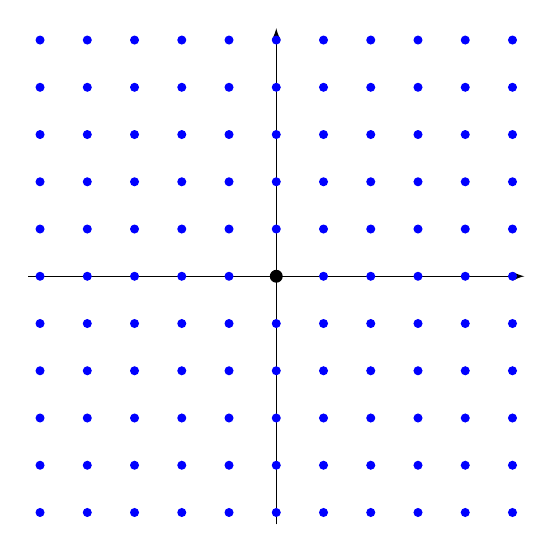
\begin{tikzpicture}[scale=0.3]
		\coordinate (Origin)   at (0,0);
		\coordinate (XAxisMin) at (-10.5,0);
		\coordinate (XAxisMax) at (10.5,0);
		\coordinate (YAxisMin) at (0,-10.5);
		\coordinate (YAxisMax) at (0,10.5);
		\draw [thin, black,-latex] (XAxisMin) -- (XAxisMax);% Draw x axis
		\draw [black,-latex] (YAxisMin) -- (YAxisMax);% Draw y axis

		\clip (-10.5,-10.5) rectangle (10.5cm,10.5cm); % Clips the picture...
		%\pgftransformcm{1}{0}{0}{1}{\pgfpoint{0cm}{0cm}}
			  % This is actually the transformation matrix entries that
			  % gives the slanted unit vectors. You might check it on
			   % MATLAB etc. . I got it by guessing.
		%\coordinate (Bone) at (0,2);
		%\coordinate (Btwo) at (2,-2);
		%\draw[style=help lines,dashed] (-10,-10) grid[step=2cm] (10,10);
			  % Draws a grid in the new coordinates.
			  %\filldraw[fill=gray, fill opacity=0.3, draw=black] (0,0) rectangle (2,2);
				  % Puts the shaded rectangle
		\foreach \x in {-5,-4,...,5}{% Two indices running over each
		  \foreach \y in {-5,-4,...,5}{% node on the grid we have drawn 
			\node[draw,circle,inner sep=1pt,fill, blue] at (2*\x,2*\y) {};
				% Places a dot at those points
		  }
		}
		\node[draw,circle,inner sep=1.5pt,fill, black] at (0,0) {};
	  \end{tikzpicture}
	  \caption{The ring of integers $\mathbb{Z}[i]$ for $\mathbb{Q}(i)$.}
	  \label{fig:gaussian-1}
	\end{figure}
	
	\begin{figure}[ht]
	\centering
	  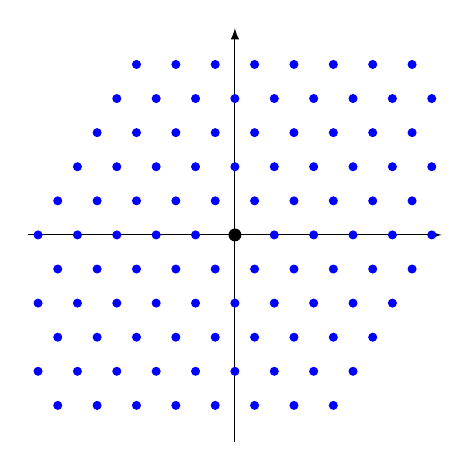
\begin{tikzpicture}[scale=0.25]
		\coordinate (Origin)   at (0,0);
		\coordinate (XAxisMin) at (-10.5,0);
		\coordinate (XAxisMax) at (10.5,0);
		\coordinate (YAxisMin) at (0,-10.5);
		\coordinate (YAxisMax) at (0,10.5);
		\draw [thin, black,-latex] (XAxisMin) -- (XAxisMax);% Draw x axis
		\draw [black,-latex] (YAxisMin) -- (YAxisMax);% Draw y axis

		\clip (-10.5,-10.5) rectangle (10.5cm,10.5cm); % Clips the picture...
		%\pgftransformcm{1}{0}{0}{1}{\pgfpoint{0cm}{0cm}}
			  % This is actually the transformation matrix entries that
			  % gives the slanted unit vectors. You might check it on
			   % MATLAB etc. . I got it by guessing.
		%\coordinate (Bone) at (0,2);
		%\coordinate (Btwo) at (2,-2);
		%\draw[style=help lines,dashed] (-10,-10) grid[step=2cm] (10,10);
			  % Draws a grid in the new coordinates.
			  %\filldraw[fill=gray, fill opacity=0.3, draw=black] (0,0) rectangle (2,2);
				  % Puts the shaded rectangle
		\foreach \x in {-5,-4,...,5}{% Two indices running over each
		  \foreach \y in {-5,-4,...,5}{% node on the grid we have drawn 
			\node[draw,circle,inner sep=1pt,fill, blue] at (2*\x+\y,1.732*\y) {};
				% Places a dot at those points
		  }
		}
		\node[draw,circle,inner sep=1.5pt,fill, black] at (0,0) {};
	  \end{tikzpicture}
	  \caption{The ring of integers $\mathbb{Z}[\frac{1+\sqrt{-3}}{2}]$ for $\mathbb{Q}(\sqrt{-3})$.}
	  \label{fig:eisenstein-1}
	\end{figure}
	
	In particular, we observe that each of these rings of integers is a lattice in $\mathbb{R}^2$.  On the other hand, $\mathbb{Q}(\sqrt{5})$ most naturally embeds into $\mathbb{R}$, not $\mathbb{R}^2$.  It turns out (not entirely obviously) that the ring of integers $\mathbb{Z}[\frac{1+\sqrt{5}}{2}]$ is dense in $\mathbb{R}$; see Figure \ref{fig:sqrt-5-1}.
	
	\begin{figure}[h]
	\centering
	  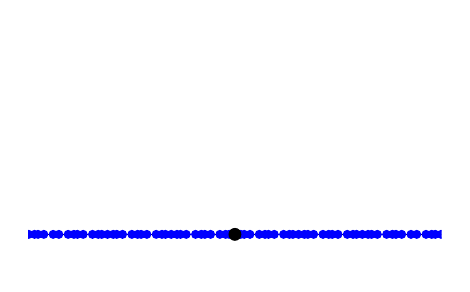
\begin{tikzpicture}[scale=0.25]
		\coordinate (Origin)   at (0,0);
		\coordinate (XAxisMin) at (-10.5,0);
		\coordinate (XAxisMax) at (10.5,0);
		\coordinate (YAxisMin) at (0,-10.5);
		\coordinate (YAxisMax) at (0,10.5);
		\draw [thin, black,-latex] (XAxisMin) -- (XAxisMax);% Draw x axis
		%\draw [black,-latex] (YAxisMin) -- (YAxisMax);% Draw y axis

		\clip (-10.5,-1.5) rectangle (10.5cm,10.5cm); % Clips the picture...
		%\pgftransformcm{1}{0}{0}{1}{\pgfpoint{0cm}{0cm}}
			  % This is actually the transformation matrix entries that
			  % gives the slanted unit vectors. You might check it on
			   % MATLAB etc. . I got it by guessing.
		%\coordinate (Bone) at (0,2);
		%\coordinate (Btwo) at (2,-2);
		%\draw[style=help lines,dashed] (-10,-10) grid[step=2cm] (10,10);
			  % Draws a grid in the new coordinates.
			  %\filldraw[fill=gray, fill opacity=0.3, draw=black] (0,0) rectangle (2,2);
				  % Puts the shaded rectangle
		\foreach \x in {-5,-4,...,5}{% Two indices running over each
		  \foreach \y in {-5,-4,...,5}{% node on the grid we have drawn 
			\node[draw,circle,inner sep=1pt,fill, blue] at (2*\x+\y+\y*2.236,0) {};
				% Places a dot at those points
		  }
		}
		\node[draw,circle,inner sep=1.5pt,fill, black] at (0,0) {};
	  \end{tikzpicture}
	  \caption{A (bad!) visualization of the ring of integers $\mathbb{Z}[\frac{1+\sqrt{5}}{2}]$ of $\mathbb{Q}(\sqrt{5})$ on the number line.}
	  \label{fig:sqrt-5-1}
	\end{figure}
	
	Our first goal is to provide a way of visualizing $\mathbb{Z}[\frac{1+\sqrt{5}}{2}]$ as a lattice, analogous to Figures \ref{fig:gaussian-1} and \ref{fig:eisenstein-1}.  For this, we need the notion of \emph{embeddings}.
	
	\begin{definition}
		A real embedding of a number field $K$ is an injective homomorphism $\sigma\colon K \hookrightarrow \mathbb{R}$.  A complex embedding of a number field $K$ is an injective homomorphism $\sigma\colon K \hookrightarrow \mathbb{C}$ that doesn't factor through an embedding to $\mathbb{R}$ (equivalently, whose image $\sigma(K)$ is not contained in $\mathbb{R}$).  An embedding of $K$ is implicitly either a real or complex embedding.
	\end{definition}
	
	We summarize several useful facts in the following lemma.
	
	\begin{lemma}\label{lem:embedding-props}
		Let $K$ be a number field of degree $n$.  Then:
		\begin{enumerate}
			\item If $\alpha \in K$ is a root of $f \in \mathbb{Q}[x]$, then so is $\sigma(\alpha)$.
			\item There are exactly $n$ embeddings of $K$.
			\item Complex embeddings come in pairs, differing by complex conjugation.  
			\item If $r_1$ denotes the number of real embeddings of $K$ and $r_2$ denotes the number of pairs of complex embeddings, then $n=r_1+2r_2$.
			\item If $\widetilde{K}$ denotes the normal closure\footnote{i.e., splitting field} of $K$, then $\mathrm{Gal}(\widetilde{K}/\mathbb{Q})$ acts faithfully and transitively on the set of embeddings of $K$.
		\end{enumerate}
	\end{lemma}
	\begin{proof}
		1) Since $\sigma$ is an injective field homomorphism, it fixes $\mathbb{Q}$.  Thus, for any $f \in \mathbb{Q}[x]$ and any $\alpha \in K$, $\sigma(f(\alpha)) = f(\sigma(\alpha))$, so $\sigma(\alpha)$ is a root of $f$ if and only if $\alpha$ is.
		
		2) Since $K$ has degree $n$, there is some $\alpha$ for which $K = \mathbb{Q}(\alpha)$ and whose minimal polynomial $f_\alpha(x)$ has degree $n$.  By part 1), $\sigma(\alpha)$ must be one of the $n$ conjugates of $\alpha$, and this choice completely determines $\sigma$ since $\sigma$ must fix $\mathbb{Q}$.  Each of these $n$ choices defines an embedding, and thus there are exactly $n$ embeddings of $K$.
		
		3) Let $\tau$ denote complex conjugation.  If $\sigma$ is a complex embedding, then $\tau \circ \sigma$ is also an embedding of $K$, necessarily not equal to $\sigma$ since $\sigma$ is complex.
		
		4) Follows from 2) and 3).
		
		5)  By 1) and 2), if $K = \mathbb{Q}(\alpha)$, then embeddings of $K$ are in correspondence with a choice $\sigma(\alpha) = \alpha_i$, where $\alpha_1,\dots,\alpha_n$ are the conjugates of $\alpha$.  Moreover, $\widetilde{K}=\mathbb{Q}(\alpha_1,\dots,\alpha_n)$, so all $\alpha_i$ are defined in $\widetilde{K}$.  An element $\phi \in \mathrm{Gal}(\widetilde{K}/\mathbb{Q})$ is a field automorphism of $\widetilde{K}$, which must send each $\alpha_i$ to some $\alpha_j$.  That is, it acts on the set $\{\alpha_1,\dots,\alpha_n\}$.  It therefore also acts in the obvious way on the set of embeddings by exploiting the correspondence between embeddings and conjugates.  
		
		A ``transitive'' action of a group $G$ on a set $\{1,\dots,n\}$ is one for which, for every pair $(i,j)$, there is an element $g \in G$ for which $g(i)=j$.  There is a field automorphism $\phi \in \mathrm{Gal}(\widetilde{K}/\mathbb{Q})$ for which $\phi(\alpha) = \alpha_i$ for any $i$, from which follows that the action of $\mathrm{Gal}(\widetilde{K}/\mathbb{Q})$ on the set of conjugates of $\alpha$ is transitive.  By the way we defined the action on the set of embeddings, it follows that the action of $\mathrm{Gal}(\widetilde{K}/\mathbb{Q})$ on the set of embeddings is also transitive.
		
		An action is ``faithful'' if only the identity element fixes everything.  The action of $\mathrm{Gal}(\widetilde{K}/\mathbb{Q})$ on the conjugates $\alpha_1,\dots,\alpha_n$ is faithful: if $\phi(\alpha_i) = \alpha_i$ for each $i$, then since $\widetilde{K}=\mathbb{Q}(\alpha_1,\dots,\alpha_n)$, $\phi$ must be the identity automorphism.  Since we have defined the action of $\mathrm{Gal}(\widetilde{K}/\mathbb{Q})$ on embeddings via its action on conjugates, it follows that the action of $\mathrm{Gal}(\widetilde{K}/\mathbb{Q})$ on the set of embeddings must be faithful as well.
	\end{proof}
	
	\begin{remark}
		There's a lot of formal manipulation going on in the statement and proof of the fifth claim.  Here's the real point.  We can abstractly construct number fields as quotients $\mathbb{Q}[x] / (f(x))$ where $f(x)$ is an irreducible polynomial, but in this formalism we haven't ``picked a root.''  For example, if $f(x)=x^2-2$, then we have formally constructed $\mathbb{Q}(\sqrt{2}) \simeq \mathbb{Q}[x]/(x^2-2)$ without having to specify which squareroot of $2$ we mean.  We can let embeddings ``choose'' a squareroot for us.  The substance of the fifth point is entirely that instead of the (very useful!) notion that the Galois group permutes roots of irreducible polynomials, it instead permutes the embeddings.  In modern number theory, it's considered gauche to fix a root when thinking about number fields.  You'll never actually be misled if you want to fix a root, but it's both psychologically and mathematically important to remember you could have made a different choice, and that embeddings create the universes in which you made that alternate choice.
	\end{remark}
\end{document}

\draw [ultra thick,-latex,red] (Origin)
			-- (Bone) node [above left] {$b_1$};
		\draw [ultra thick,-latex,red] (Origin)
			-- (Btwo) node [below right] {$b_2$};
		\draw [ultra thick,-latex,red] (Origin)
			-- ($(Bone)+(Btwo)$) node [below right] {$b_1+b_2$};
		\draw [ultra thick,-latex,red] (Origin)
			-- ($2*(Bone)+(Btwo)$) node [above left] {2$b_1+b_2$};
		\filldraw[fill=gray, fill opacity=0.3, draw=black] (Origin)
			rectangle ($2*(Bone)+(Btwo)$);
		%\draw [thin,-latex,red, fill=gray, fill opacity=0.3] (0,0)
			% -- ($2*(0,2)+(2,-2)$)
			% -- ($3*(0,2)+2*(2,-2)$) -- ($(0,2)+(2,-2)$) -- cycle;
